% 
%            ,,                                        
%          `7MM            _.o9                                
%            MM                                             
%  ,6"Yb.    MM  ,p6"bo   ,6"Yb.  M"""MMV  ,6"Yb.  `7Mb,od8 
% 8)   MM    MM 6M'  OO  8)   MM  '  AMV  8)   MM    MM' "' 
%  ,pm9MM    MM 8M        ,pm9MM    AMV    ,pm9MM    MM     
% 8M   MM    MM YM.    , 8M   MM   AMV  , 8M   MM    MM     
% `Moo9^Yo..JMML.YMbmd'  `Moo9^Yo.AMMmmmM `Moo9^Yo..JMML.   
% 
% 
% Free and Open-Source template for academic works
% https://github.com/dpmj/alca

\begin{small}
\begin{Verbatim}[commandchars=\\\{\}]

\end{Verbatim}
\end{small}

{\small \verb|a|}


\clearpage
\cleardoublepage

\chapter{Considerazioni di MLSecOps}

Come accennato nei Capitoli 1 e 2, il paradigma MLSecOps è di complessa implementazione, specialmente se si interseca col articolato mondo delle architetture a microservizi. In generale, con "MLSecOps" intendiamo un insieme di tecniche e metodologie per applicare principi di sicurezza alle pipeline, alle infrastrutture e ai prodotti software relativi al machine learning.

Un contributo originale di questa tesi di laurea magistrale è rappresentato dalla creazione parallela di un'architettura (del tutto simile a quella descritta nel Capitolo 4) infetta e vulnerabile a specifici tipi di attacchi, oltre che all'analisi compilativa di pratiche relativamente meno dannose, come il load testing.

\begin{figure}[H]
    \centering
    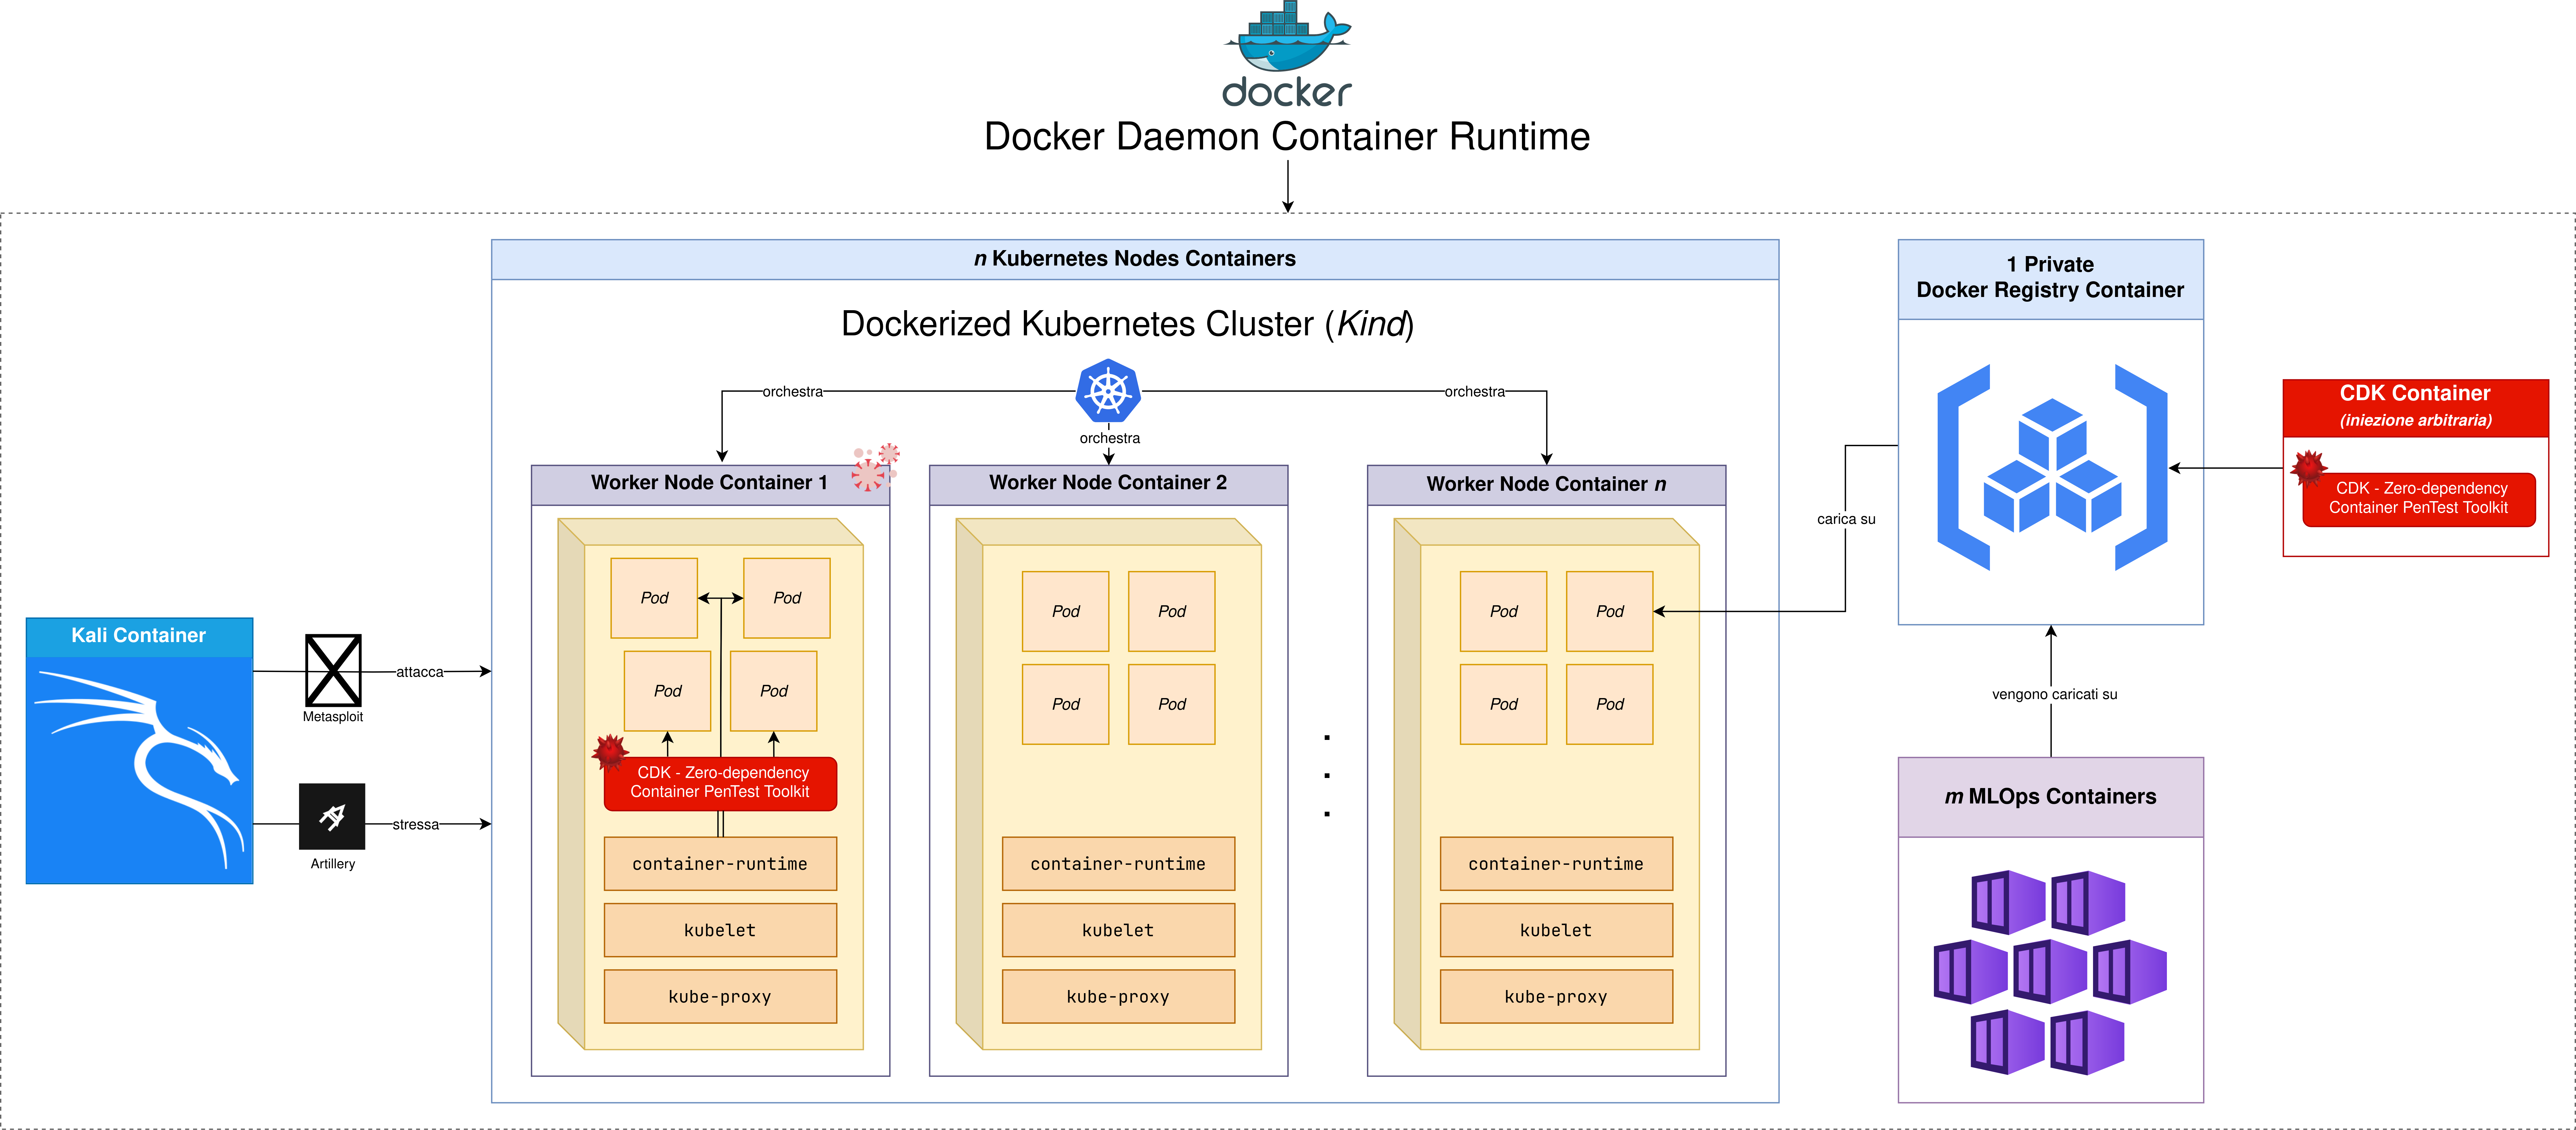
\includegraphics[width=\linewidth]{figures/ch4and5/arch2.png}
    \caption[Anteprima dell'architettura infetta realizzata]{Anteprima dell'architettura infetta realizzata}
    \label{fig:cha6:arch}
\end{figure}

Poiché l'architettura è generata in locale mediante Kind, il quale produce dei container Docker per ogni nodo del cluster Kubernetes, allo stesso modo dovremmo immaginare degli avversari - più o meno sofisticati - containerizzati sul proprio host. Nella fattispecie, sono stati immaginati i seguenti scenari:

\begin{itemize}
    \item Un avversio \glsname{kali} che, utilizzando \glsname{metasploit}, effettua diversi tipi di attacco dall'esterno dell'infrastruttura \glsname{kubernetes}.
    \item Un avversario che, con l'obiettivo di rendere vulnerabile il cluster, produce un'immagine \glsname{docker} di \glsname{cdk} da caricare sul registro Docker on-prem dell'architettura, che sarà poi iniettabile in un pod Kubernetes durante una tipica esecuzione delle pipeline di \glsname{kubeflow}, posto che l'avversario abbia sufficienti permessi (nel contesto RBAC del sistema) per realizzare o manipolare i componenti Kubeflow.
    \item Un avversario che, post-mortem, effettua una escalation all'interno di un node del cluster Kubernetes usando CDK.
    \item Un avversario, oppure una parte onesta, che effettua load testing contro il Control Plane di Kubernetese, utilizzando \glsname{artillery}. L'obiettivo di questo attacco (in genere simulato) è di valutare la resilienza del sistema.
\end{itemize}

\section{Kali Linux}

Kali Linux, un sistema operativo basato su Debian progettato specificamente per le attività di penetration testing e sicurezza informatica, si presenta come una risorsa essenziale nell'arsenale di professionisti della sicurezza. La sua forza risiede nella vasta gamma di strumenti preinstallati, mirati a facilitare e ottimizzare le attività di test della sicurezza e analisi forense. Da una prospettiva accademica, Kali Linux si configura come un ambiente robusto e specializzato che favorisce la comprensione approfondita delle metodologie di test della sicurezza, fornendo agli studenti un terreno fertile per acquisire competenze pratiche nell'ambito della sicurezza informatica \cite{kali_linux_overview}.

Gli strumenti inclusi in Kali Linux coprono una vasta gamma di ambiti, dalla scansione di reti e individuazione di vulnerabilità alla forensica digitale. Un esempio di strumento emblematico è Metasploit, un framework di penetration testing che agevola lo sviluppo, il test e la distribuzione di exploit. Il suo utilizzo consente agli esperti di sicurezza di simulare attacchi e valutare l'efficacia delle difese, fornendo una panoramica approfondita delle possibili minacce che potrebbero compromettere la sicurezza di un sistema \cite{metasploit_paper}.

Un esempio pratico di utilizzo di Metasploit in Kali Linux può essere espresso attraverso il seguente snippet di codice. Il comando seguente avvia Metasploit e stabilisce una connessione con un host remoto attraverso un exploit specifico:

\begin{small}
\begin{Verbatim}[commandchars=\\\{\}]
msfconsole
use exploit/windows/smb/ms17_010_eternalblue
set RHOSTS <indirizzo_ip_obiettivo>
exploit
\end{Verbatim}
\end{small}

Questo esempio illustra la semplicità con cui gli strumenti di Kali Linux, come Metasploit, possono essere impiegati per condurre attività di penetration testing su reti e sistemi, evidenziando il valore intrinseco di questi strumenti per gli esperti di sicurezza \cite{kali_metasploit_integration}.

In conclusione, Kali Linux, con la sua vasta gamma di strumenti dedicati alla sicurezza informatica, costituisce una risorsa fondamentale per gli studiosi e gli operatori di sicurezza. L'integrazione di strumenti avanzati come Metasploit offre opportunità senza precedenti per esplorare, comprendere e mitigare le minacce digitali, contribuendo significativamente alla formazione accademica e pratica nel campo della sicurezza informatica \cite{kali_linux_education}.

\subsection{Containerizzazione di Kali Linux e interazione con l'host}

Orientativamente, operando su un cluster locale Kind abbiamo la necessità di simulare mediante Docker un avversario Kali Linux, containerizzando il sistema operativa assieme agli strumenti che vorremmo utilizzare, come Metasploit. La documentazione ufficiale di Kali Linux a tal riguardo invita a produrre una propria immagine Docker personalizzata per generare on-the-fly un container con gli strumenti richiesti, o in alternativa installarli ogni volta che si spegne e ricrea il container.

E' stato quindi prodotto un Dockerfile per produrre un'immagine Docker comprensiva di tutti gli strumenti necessari per i nostri fini.

\begin{code}
\captionof{listing}{Kali Linux Dockerfile}
\label{code:apx:a:dockerfile}
\begin{minted}{dockerfile}
# Produce un'immagine Docker di Kali Linux per le analisi di Container Security e l'esecuzione di attacchi di Penetration Testing.
# Fare riferimento alla documentazione del progetto per maggiori dettagli.

FROM kalilinux/kali-rolling

WORKDIR /root
ENV DEBIAN_FRONTEND=noninteractive

# L'immagine di Kali Linux non include di default il pacchetto kali-linux-headless ..
# .. che contiene la maggior parte degli strumenti di analisi e attacco.
# Rif. https://www.kali.org/docs/containers/using-kali-docker-images/

RUN apt -y update && \
    apt -y dist-upgrade && \
    apt -y autoremove && \
    apt clean && \
    apt -y install wget

# Siamo interessati esclusivamente a Metasploit Framework, contenuto nel pacchetto kali-linux-top10.
# Immagini più organiche potrebbero utilizzare il pacchetto kali-linux-all.
# Rif. https://www.kali.org/blog/kali-linux-metapackages/

RUN apt -y install -f kali-tools-top10

# Iniezione arbitraria del binario del Zero Dependency Container Penetration Toolkit
# Rif. https://github.com/cdk-team/CDK

RUN wget https://github.com/cdk-team/CDK/releases/download/v1.5.2/cdk_linux_amd64 && \
    chmod a+x cdk_linux_amd64 && \
    mv cdk_linux_amd64 /usr/local/bin/cdk
\end{minted}
\end{code}

E' rapidamente osservabile come l'immagine Docker di Kali sia stata caricata anche con dei binari di CDK. Per costruire l'immagine, è sufficiente eseguire il seguente comando:

\begin{small}
\begin{Verbatim}[commandchars=\\\{\}]
\textcolor{blue}{docker} build -t kali-cdk \\ 
    --file=container-sec/kali.Dockerfile \\ 
    container-sec
\end{Verbatim}
\end{small}

Infine, per eseguire Kali Linux:

\begin{small}
\begin{Verbatim}[commandchars=\\\{\}]
\textcolor{blue}{docker} run --network=host -i --tty kali-cdk
\end{Verbatim}
\end{small}

Si invita a porre particolare attenzione alla network flag (host) indicata nel comando. Questa flag permette all'avversario containerizzato Kali di interagire col cluster Kind che, chiaramente, opera su container diversi sulla propria macchina.

\section{Metasploit Framework}

Metasploit, una pietra miliare nell'arsenale degli specialisti di sicurezza informatica, si presenta come un framework di penetration testing open-source ampiamente utilizzato per condurre test di penetrazione e sviluppare exploit. La sua notevole popolarità è attribuibile alla sua vasta gamma di moduli, payload e strumenti integrati, fornendo agli esperti di sicurezza un ambiente flessibile e potente per esplorare le vulnerabilità dei sistemi. Metasploit si distingue per la sua capacità di automatizzare complesse procedure di penetration testing, consentendo agli operatori di sicurezza di identificare e correggere le vulnerabilità in modo efficiente e mirato \cite{metasploit_framework}.

\begin{figure}[H]
    \centering
    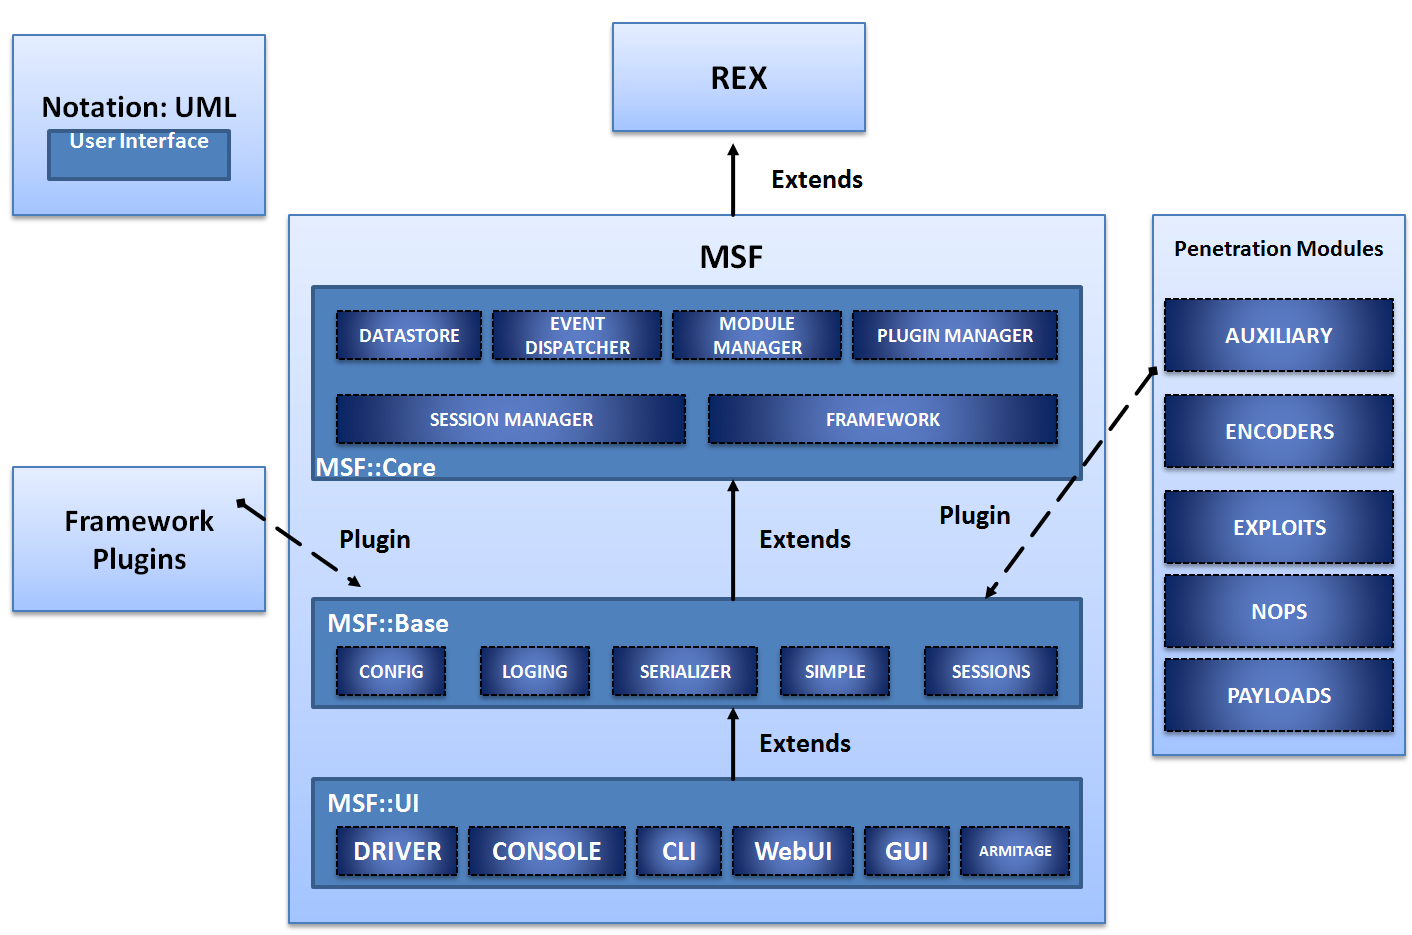
\includegraphics[width=\linewidth]{figures/ch4and5/msf.png}
    \caption[Architettura di Metasploit]{Architettura di Metasploit}
    \label{fig:cha6:msf}
\end{figure}

L'architettura modulare di Metasploit è un elemento chiave del suo successo. I moduli di Metasploit, detti "exploit", si concentrano su specifiche vulnerabilità o servizi, facilitando agli operatori di selezionare gli strumenti più adatti al contesto di test. Questo approccio modulare conferisce a Metasploit una notevole flessibilità, consentendo di adattarsi a una vasta gamma di scenari di sicurezza, dalla valutazione di vulnerabilità a simulazioni di attacchi realistici \cite{metasploit_modularity}.

Metasploit, con la sua potente architettura modulare e la vasta comunità di utenti e sviluppatori, continua a essere uno degli strumenti più rilevanti per condurre test di penetrazione e valutare la sicurezza dei sistemi. La sua versatilità, facilità d'uso e capacità di automatizzazione lo rendono uno strumento cruciale per gli esperti di sicurezza impegnati nella protezione delle infrastrutture digitali da minacce sempre più sofisticate \cite{metasploit_future}.

Il container Kali verrà utilizzato prevalentemente come base di appoggio per il software Metasploit. In particolare, verranno utilizzati i moduli del catalogo "Kubernetes Penetration Testing" al fine di esporre le vulnerabilità del cluster Kind. Si tratta, in particolare, dei seguenti moduli: {\small \verb|kubernetes/enum|} e {\small \verb|kubernetes/exec|}.

Verrà mostrato un uso esemplificativo del primo modulo, poiché il secondo - venendo prevalentemente utilizzato in contesti di shell execution - non si presta al contesto di Kubeflow, in cui i pods sono Jobs one-shot che muoiono al termine dell'esecuzione.

Per impiegare questi moduli, bisognerà prima di tutto generare un Service Account da affibbiare ad un ipotetico amministratore del cluster compromesso. Questa procedura è delineata nella sezione "Access Clusters Using the Kubernetes API" \cite{k8s-docs-access} della documentazione di Kubernetes. In particolare, è sufficiente eseguire i seguenti comandi:

\begin{small}
\begin{Verbatim}[commandchars=\\\{\}]
\textcolor{purple}{kubectl} create -n default serviceaccount \\
    admin-sa --dry-run=client -o yaml | \textcolor{purple}{kubectl} apply -f -

\textcolor{purple}{kubectl} create -n default clusterrolebinding \\
    admin-sa-binding --clusterrole=cluster-admin \\
    --serviceaccount=default:admin-sa --dry-run=client -o yaml \\
    | \textcolor{purple}{kubectl} apply -f -

\textcolor{purple}{kubectl} create token admin-sa
\end{Verbatim}
\end{small}

Il processo genererà un JSON Web Token (JWT) di un cluster admin con accesso completo alle risorse del sistema. In particolare, l'ultimo comando dovrebbe restituire un (JWT) necessario per autenticarsi al cluster Kubernetes. Il JWT dovrebbe avere una forma di questo tipo:

\begin{code}
\captionof{listing}{JSON Web Token esemplificativo}
\label{code:apx:a:dockerfile}
\begin{minted}{dockerfile}
eyJhbGciOiJSUzI1NiIsImtpZCI6IjFHQW1LbjY3U2kyNTZod0s4Q2VldWtyYnRiM2Q0Wnpi
[..] Il JWT prosegue [..]
\end{minted}
\end{code}

La validità del JWT è verificabile online con tool ben noti come {\small \verb|jwt.io|}.

\begin{figure}[H]
    \centering
    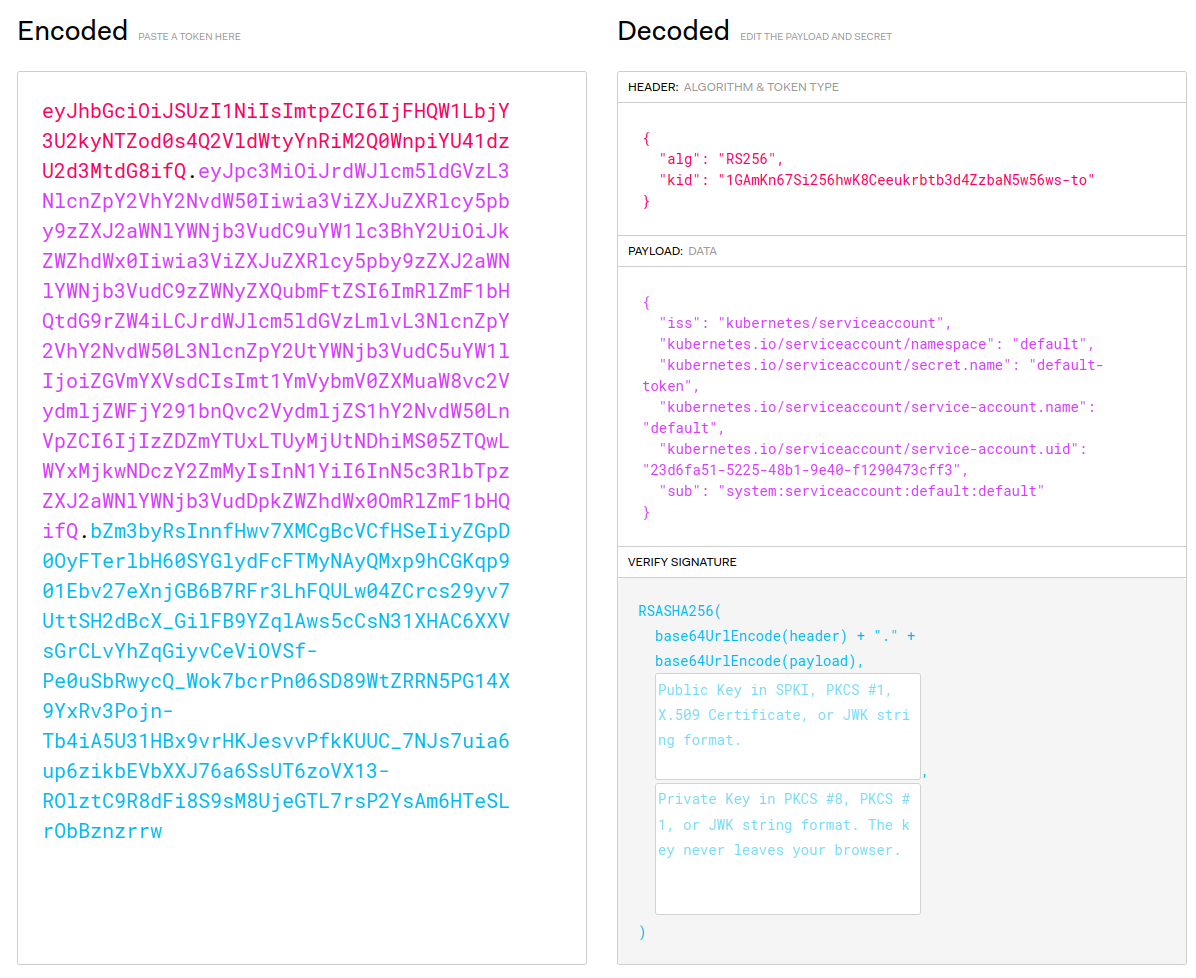
\includegraphics[width=\linewidth]{figures/ch4and5/jwt.png}
    \caption[Validità del JSON Web Token]{Validità del JSON Web Token}
    \label{fig:cha6:jwt}
\end{figure}

Se il JWT risulta valido, sarà possibile procedere con gli exploit.

\subsection{Kubernetes Resource Enumeration}

Il modulo {\small \verb|enum|} viene usato per enumerare le risorse del cluster, e in particolare i pod. Tutte le risorse vengono accluse all'exploit, fra cui Namespaces, DaemonSets, ReplicaSets e Deployments. Ad esempio, lanciando l'exploit è possibile visionare i pod del NVIDIA GPU Operator installato nel Capitolo 4 per integrare il supporto al runtime CUDA.

Per enumerare le risorse Kubernetes, seguire i seguenti passaggi:

\begin{itemize}
    \item Accedere a Kali con {\small \verb|docker run --network=host -i --tty kali-cdk|}
    \item Accedere alla shell di Metasploit digitando {\small \verb|msfconsole|}
    \item Accedere al modulo di exploit digitando {\small \verb|use auxiliary/scanner/http/kubernetes_enum|}
    \item Impostare l'endpoint dell'API Server di Kubernetes con {\small \verb|set RHOST https://127.0.0.1:39175|}
    \item Impostare il JWT digitando {\small \verb|set TOKEN <JWT>|} e sostituendo {\small \verb|<JWT>|} con il JWT generato in precedenza
    Eseguire l'exploit con {\small \verb|run|}
\end{itemize}

Il software dovrebbe restituire esattamente le stesse risorse che si otterrebbero con {\small \verb|kubectl get all|}, mappando 1:1 l'infrastruttura Kubernetes presente sul sistema. Un log di esempio è disponibile in {\small \verb|/container-sec/logs|}.

\begin{code}
\captionof{listing}{Kubernetes Resource Enumeration}
\label{code:apx:a:yaml}
\begin{minted}{yaml}
Secrets (namespace: default)
============================

    #   namespace  name                                        type                                 data                    age
    -   ---------  ----                                        ----                                 ----                    ---
    0   default    default-token                               kubernetes.io/service-account-token  ca.crt,namespace,token  57m
    1   default    kubernetes-dashboard-certs                  Opaque                                                       14m
    2   default    kubernetes-dashboard-csrf                   Opaque                               csrf                    14m
    3   default    kubernetes-dashboard-key-holder             Opaque                               priv,pub                14m
    4   default    secrets-basic-auth                          kubernetes.io/basic-auth             password,username       14m
    5   default    secrets-dockerconfigjson                    kubernetes.io/dockerconfigjson       .dockerconfigjson       14m
    6   default    secrets-empty                               Opaque                                                       14m
    7   default    secrets-id-ed25519-with-passphrase          kubernetes.io/ssh-auth               ssh-privatekey          14m
    8   default    secrets-id-ed25519-without-passphrase       kubernetes.io/ssh-auth               ssh-privatekey          14m
    9   default    secrets-id-rsa-with-passphrase              kubernetes.io/ssh-auth               ssh-privatekey          14m
    10  default    secrets-id-rsa-without-passphrase           kubernetes.io/ssh-auth               ssh-privatekey          14m
    11  default    secrets-tls                                 kubernetes.io/tls                    tls.crt,tls.key         14m
    12  default    secrets-user-password                       Opaque                               password,username       14m
    13  default    sh.helm.release.v1.kubernetes-dashboard.v1  helm.sh/release.v1                   release                 14m

Pods (namespace: gpu-operator)
==============================

    #  namespace     name                                                             status     containers                                                                                       ip
    -  ---------     ----                                                             ------     ----------                                                                                       --
    0  gpu-operator  gpu-feature-discovery-4bhjw                                      Running    gpu-feature-discovery (image: nvcr.io/nvidia/gpu-feature-discovery:v0.8.2-ubi8)                  10.244.0.25
    1  gpu-operator  gpu-operator-1699611486-node-feature-discovery-gc-6689cc7dpk5r5  Running    gc (image: registry.k8s.io/nfd/node-feature-discovery:v0.14.2)                                   10.244.0.20
    2  gpu-operator  gpu-operator-1699611486-node-feature-discovery-master-8654k5wdn  Running    master (image: registry.k8s.io/nfd/node-feature-discovery:v0.14.2 TCP:8080,TCP:8081)             10.244.0.19
    3  gpu-operator  gpu-operator-1699611486-node-feature-discovery-worker-68ml2      Running    worker (image: registry.k8s.io/nfd/node-feature-discovery:v0.14.2 TCP:8081)                      10.244.0.15
    4  gpu-operator  gpu-operator-c68996868-8ckrj                                     Running    gpu-operator (image: nvcr.io/nvidia/gpu-operator:v23.9.0 TCP:8080)                               10.244.0.22

[..] I log continuano [..]
\end{minted}
\end{code}

Intuitivamente, questo attacco è molto simile ad un network mapping, in cui si enumerano le componenti di rete. In maniera del tutto analoga, tramite questo modulo siamo in grado di avere una visione completa e organica delle risorse del cluster.

\section{Zero-dependency Container Penetration Testing Toolkit (CDK)}

Il panorama sempre dinamico della sicurezza informatica richiede strumenti avanzati e agili per condurre test di penetrazione efficaci. In questo contesto, emerge lo Zero-dependency Container Penetration Testing Toolkit (\glsname{cdk}), un'innovativa risorsa che si distingue per la sua modularità e versatilità nell'affrontare sfide complesse di sicurezza dei container. CDK si configura come una soluzione all'avanguardia, progettata per eliminare dipendenze esterne, garantendo così un'implementazione agevole e una portabilità senza precedenti. Questa caratteristica lo rende particolarmente adatto per ambienti containerizzati, fornendo agli operatori di sicurezza uno strumento flessibile e leggero per la valutazione della sicurezza \cite{cdk_overview}.

Un elemento distintivo di CDK è la sua capacità di adattarsi a diverse architetture di container senza richiedere dipendenze esterne, conferendo agli esperti di sicurezza la possibilità di condurre test di penetrazione senza oneri aggiuntivi. Questa caratteristica unica è fondamentale, soprattutto considerando l'eterogeneità delle infrastrutture containerizzate moderne. CDK permette agli operatori di esplorare, analizzare e valutare la sicurezza dei container senza le limitazioni spesso associate alle dipendenze esterne, garantendo così un approccio di testing agnostico e scalabile \cite{cdk_modularity}.

L'architettura modulare di CDK è fondamentale per la sua efficacia nel contesto dei test di penetrazione. Ogni modulo di CDK si concentra su aspetti specifici della sicurezza, consentendo agli operatori di selezionare e integrare solo le funzionalità necessarie per il contesto di test in esame. Questo approccio mirato non solo semplifica l'implementazione, ma ottimizza anche le risorse, garantendo che gli operatori possano concentrarsi sulle aree di maggiore rilevanza senza l'ingombro di funzionalità superflue \cite{cdk_modularity}.

Lo Zero-dependency Container Penetration Testing Toolkit (CDK) si rivela un alleato inestimabile nell'ambito della sicurezza dei container. La sua natura priva di dipendenze esterne, l'architettura modulare e la facilità d'uso lo posizionano al centro delle pratiche di testing di penetrazione, offrendo agli operatori uno strumento potente e flessibile per affrontare le sfide sempre crescenti della sicurezza informatica in ambienti containerizzati \cite{cdk_future}.

\subsection{Containerizzazione di CDK e iniezione arbitraria su un registro Docker}

E' stata realizzata un'immagine Docker che monta il toolkit CDK su base Alpine. Per costruirla e caricarla sul Docker Registry on-prem, eseguire il seguente comando.

\begin{small}
\begin{Verbatim}[commandchars=\\\{\}]
\textcolor{blue}{docker} build \\
    -t localhost:5000/cdk \\
    --file=container-sec/cdk.Dockerfile \\
    container-sec && \
\textcolor{blue}{docker} push \\
    localhost:5001/step-dataset-generation-config:latest
\end{Verbatim}
\end{small}

L'mmagine può essere iniettata arbitrariamente nel cluster Kubernetes, sul nodo kind-control-plane, producendo un nuovo pod all'interno dello stesso, col fine ultimo di eseguire attacchi di Penetration Testing. Per farlo, eseguire il seguente comando.

\begin{small}
\begin{Verbatim}[commandchars=\\\{\}]
\textcolor{purple}{kubectl} debug node/kind-control-plane \\
    -it \\
    --image=localhost:5001/cdk
\end{Verbatim}
\end{small}

Questo approccio, per quanto indagato, non è stato approfondito ulteriormente, poiché strettamente vincolato alla capacità dell'avversario di iniettare immagini corrotta nel registro, ed eseguire un pull malizioso, e cioè - in generale - di forgiare componenti Kubeflow.

\begin{code}
\captionof{listing}{Dockerfile di CDK}
\label{code:apx:a:dockerfile}
\begin{minted}{dockerfile}
# Produce un'immagine Docker di CDK.
# Rif. https://github.com/cdk-team/CDK

FROM alpine

RUN apk add --no-cache wget && \
    wget https://github.com/cdk-team/CDK/releases/download/v1.5.2/cdk_linux_amd64 && \
    chmod a+x cdk_linux_amd64 && \
    mv cdk_linux_amd64 /usr/local/bin/cdk
\end{minted}
\end{code}

\subsection{Creare un nodo Kind contagiato da CDK}

Durante l'installazione del sistema descritta nei capitoli precedenti, è stato eseguito uno shell script {\small \verb|(boot-kind-gpu.sh)|} per generare il cluster Kubernetes con Kind. Tale script, per rappresentare i nodi del cluster, utilizza l'immagine Docker {\small \verb|kindest/node|}. E' invece possibile generare un cluster Kind corrotto, popolato da nodi infetti col toolkit CDK, sfruttando un'immagine Docker personalizzata chiamata {\small \verb|kind-cdk|} e realizzata contestualmente a questo lavoro di tesi. Costruendo il cluster in questo modo, è possibile indagare le difese del cluster Kubernetes, e in particolare del nodo {\small \verb|kind-control-plane|} infetto, eseguendo valutazioni di Information Gathering con CDK.

Per costruire l'immagine Docker {\small \verb|kind-cdk|}, eseguire il seguente comando.

\begin{small}
\begin{Verbatim}[commandchars=\\\{\}]
\textcolor{blue}{docker} build \\
    -t kind-cdk \\
    --file=container-sec/kind.Dockerfile \\
    container-sec
\end{Verbatim}
\end{small}

A questo punto, è possibile reiterare le stesse operazioni descritte nel capitolo Installazione del sistema, avendo però cura di utilizzare lo shell script {\small \verb|boot-kind-gpu-cdk.sh|} invece di {\small \verb|boot-kind-gpu.sh|}. Lo script produrrà un cluster Kind chiamato {\small \verb|kind-cdk|} associabile a {\small \verb|kubectl|} col comando {\small \verb|kubectl cluster-info --context kind-kind-cdk|}.

Conclusa l'installazione, sarà possibile accedere al control plane di Kubernetes col seguente comando, per poi confermare che CDK sia attivo usando il comando {\small \verb|cdk|}.

\begin{small}
\begin{Verbatim}[commandchars=\\\{\}]
\textcolor{blue}{docker} exec -it kind-control-plane sh
\end{Verbatim}
\end{small}

\begin{code}
\captionof{listing}{Dockerfile di un nodo Kind contagiato da CDK}
\label{code:apx:a:dockerfile}
\begin{minted}{dockerfile}
# Produce un'immagine Docker di un worker node di Kind personalizzata per ospitare un'istanza di CDK.

FROM kindest/node:v1.27.3

# Iniezione arbitraria del binario del Zero Dependency Container Penetration Toolkit
# Rif. https://github.com/cdk-team/CDK

RUN apt update && \
    apt -y install wget && \
    wget https://github.com/cdk-team/CDK/releases/download/v1.5.2/cdk_linux_amd64 && \
    chmod a+x cdk_linux_amd64 && \
    mv cdk_linux_amd64 /usr/local/bin/cdk
\end{minted}
\end{code}

E' adesso possibile individuare le debolezze note del container con {\small \verb|cdk eva|}. E' immediantamente osservabile che il nodo risulta vulnerabile sotto molteplici aspetti, così come segnalato dal toolkit. Ad esempio, risultano esposte alcune variabili d'ambiente e file di configurazione che potrebbero essere sfruttate per un escalation.

\begin{code}
\captionof{listing}{Logs di CDK}
\label{code:apx:a:yaml}
\begin{minted}{yaml}
[  Information Gathering - Services  ]
2023/11/13 11:49:46 sensitive env found: container=docker
2023/11/13 11:49:46 sensitive env found: KUBECONFIG=/etc/kubernetes/admin.conf

[..]

cat /etc/kubernetes/admin.conf

users:
- name: kubernetes-admin
  user:
    client-certificate-data: [..]
    client-key-data: [..]
\end{minted}
\end{code}

Il file di log prodotto da cdk eva a partire da un nodo Kind vergine è disponibile nella directory {\small \verb|/container-sec/logs|} della repository di tesi.

\section{Artillery}

Il Load Testing rappresenta una pratica cruciale nel contesto della valutazione delle prestazioni di un sistema, mirando a comprendere la sua capacità di gestire carichi di lavoro variabili e, di conseguenza, fornire una base solida per l'ottimizzazione delle risorse e la garantia delle performance desiderate. Questa metodologia, intrinsecamente legata all'ingegneria del software, diviene ancor più rilevante nell'ambito della sicurezza operativa di Machine Learning (MLSecOps), dove il corretto funzionamento dei modelli di machine learning è essenziale per garantire la sicurezza e l'affidabilità dei sistemi intelligenti \cite{load_testing_overview}.

Artillery, quale strumento di Load Testing, si distingue per la sua flessibilità e versatilità nell'esecuzione di test su applicazioni web e servizi API, nonché nella simulazione di carichi di lavoro distribuiti. Nel contesto di MLSecOps, Artillery assume una rilevanza particolare, consentendo di valutare la resilienza di un sistema di machine learning sotto stress simulato. La capacità di Artillery di generare carichi di lavoro variabili e analizzare le metriche di prestazione offre una visione approfondita sul comportamento del sistema, aiutando gli operatori di sicurezza a identificare possibili vulnerabilità o punti di debolezza che potrebbero essere sfruttati da attacchi malevoli \cite{artillery_overview}.

Un esempio di utilizzo di Artillery nel contesto di MLSecOps può essere evidenziato attraverso il seguente snippet di codice YAML, che definisce un semplice scenario di test:

\begin{code}
\captionof{listing}{Esempio di load test con Artillery}
\label{code:apx:a:yaml}
\begin{minted}{yaml}
config:
target: 'https://ml-system-endpoint'
phases:
    - duration: 600
    arrivalRate: 5

scenarios:
- flow:
    - get:
        url: '/predict'

\end{minted}
\end{code}

Questo snippet configura un test in cui simuliamo un carico di lavoro costante di 5 richieste al secondo per un periodo di 600 secondi, con ciascuna richiesta che chiama l'endpoint '/predict' del sistema di machine learning. Questa rappresentazione concettuale evidenzia la capacità di Artillery di modellare scenari di carico di lavoro realistici e personalizzabili, rivelando così la sua utilità nell'ambito di MLSecOps \cite{artillery_configuration}.

L'adozione di strumenti di Load Testing, come Artillery, riveste una rilevanza cruciale nell'ambito di MLSecOps, permettendo la valutazione robusta della resilienza dei sistemi di machine learning sotto vari carichi di lavoro simulati. L'integrazione di tali pratiche all'interno delle operazioni di sicurezza contribuisce significativamente alla costruzione di sistemi intelligenti affidabili e resilienti di fronte alle sfide operative e di sicurezza che caratterizzano il panorama contemporaneo delle tecnologie intelligenti \cite{mlsecops_load_testing}.

\subsection{Kubernetes Control Plane Load Testing}

Contestualmente a questo lavoro di tesi, è stato indagato come un attacco di load testing con Artillery possa essere condotto control il Control Plane di Kubernetes, elemento centrale nell'architettura del sistema. E' stato realizzato un manifesto YAML per effettuare un blitz ai danni del Control plane, con lo scopo ultimo di analizzare i tempi di risposta e la sua inerente resilienza. 

Per farlo, eseguire il seguente comando, che avvierà un container Docker e alla fine del testing restituirà le metriche di esecuzione in {\small \verb|/container-sec/logs|}.

\begin{small}
\begin{Verbatim}[commandchars=\\\{\}]
    \textcolor{blue}{docker} run --rm -it --network=host -v \\
        ${PWD}/container-sec:/container-sec artilleryio/artillery:latest run \\
        --insecure -o /container-sec/logs/artillery-results.csv /container-sec/ \\
        k8s-api-blitz.yaml
\end{Verbatim}
\end{small}

Questo tipo di attacco può essere particolarmente utile per valutare la resilienza del control plane, e la sua esigenza di essere ridondato e posto davanti ad un load balancer.

\begin{code}
\captionof{listing}{Kubernetes Control Plane Blitz}
\label{code:apx:a:yaml}
\begin{minted}{yaml}
# Questo script di load testing può essere usato per stressare il control plan di Kubernetes.

config:
    # Kind - K8s Control Plane API Server
    target: https://127.0.0.1:39175
    phases:
    - duration: 10 # secondi
        # Definisce il numero (graduale) di "virtual users" .. 
        # .. che eseguiranno interamente gli scenari descritti.
        # Rif. https://www.artillery.io/docs/get-started/core-concepts
        arrivalRate: 1
        rampTo: 5
        name: "K8s - Warm Up"
    - duration: 20
        arrivalRate: 5
        rampTo: 10
        name: "K8s - Stretch"
    - duration: 20
        arrivalRate: 10
        rampTo: 20
        name: "K8s - Escalate"
scenarios:
    - flow:
    - loop:
        - get:
            url: "/"
        # Le interfacce pubbliche di Kubernetes sono raggruppate in namespaces.
        # Rif. https://kubernetes.io/docs/concepts/overview/kubernetes-api/
        - get:
            url: "/api/v1"
        - get:
            url: "/openapi/v2"
\end{minted}
\end{code}

Come è possibile notare, il "blitz" è composto da tre fasi di attacco, ognuna delle quali aumenta radicalmente il numero di utenti virtuali (i.e. fonti da cui partono le richieste HTTP) che operano contro il control plane. Ovviamente, in un contesto di produzione il blitz indicato avrebbe una forma più organica, con valori meglio tarati in base all'infrastruttura utilizzata (e.g. un cloud provider o altre soluzioni).

Poiché, nel caso di questa tesi, si sta adoperando Kind per sviluppare in locale, è bene ricordare che il load testing avviene {\em contro sé stessi}.

\begin{code}
\captionof{listing}{Logs di un generico blitz Artillery contro Kubernetes}
\label{code:apx:a:yaml}
\begin{minted}{yaml}
Phase started: K8s - Warm Up (index: 0, duration: 10s) 08:30:24(+0000)
Phase completed: K8s - Warm Up (index: 0, duration: 10s) 08:30:34(+0000)
Phase started: K8s - Stretch (index: 1, duration: 20s) 08:30:34(+0000)
Phase completed: K8s - Stretch (index: 1, duration: 20s) 08:30:54(+0000)
Phase started: K8s - Escalate (index: 2, duration: 20s) 08:30:54(+0000)

--------------------------------------
Metrics for period to: 08:30:30(+0000) (width: 4.747s)
--------------------------------------

http.codes.403: ................................................................ 24160
http.downloaded_bytes: ......................................................... 4469600
http.request_rate: ............................................................. 7137/sec
http.requests: ................................................................. 24169
http.response_time:
    min: ......................................................................... 0
    max: ......................................................................... 13
    mean: ........................................................................ 0.4
    median: ...................................................................... 0
    p95: ......................................................................... 1
    p99: ......................................................................... 2
http.responses: ................................................................ 24160
vusers.created: ................................................................ 9
vusers.created_by_name.0: ...................................................... 9


--------------------------------------
Metrics for period to: 08:30:40(+0000) (width: 9.999s)
--------------------------------------

http.codes.403: ................................................................ 107464
http.downloaded_bytes: ......................................................... 19880840
http.request_rate: ............................................................. 12760/sec
http.requests: ................................................................. 107510
http.response_time:
    min: ......................................................................... 0
    max: ......................................................................... 81
    mean: ........................................................................ 1.4
    median: ...................................................................... 1
    p95: ......................................................................... 4
    p99: ......................................................................... 7
http.responses: ................................................................ 107464
vusers.created: ................................................................ 49
vusers.created_by_name.0: ...................................................... 49


Phase completed: K8s - Escalate (index: 2, duration: 20s) 08:31:14(+0000)

--------------------------------------
Metrics for period to: 08:30:50(+0000) (width: 9.999s)
--------------------------------------

http.codes.403: ................................................................ 122073
http.downloaded_bytes: ......................................................... 22583320
http.request_rate: ............................................................. 13219/sec
http.requests: ................................................................. 122145
http.response_time:
    min: ......................................................................... 0
    max: ......................................................................... 166
    mean: ........................................................................ 3.7
    median: ...................................................................... 3
    p95: ......................................................................... 10.1
    p99: ......................................................................... 16
http.responses: ................................................................ 122073
vusers.created: ................................................................ 75
vusers.created_by_name.0: ...................................................... 75
\end{minted}
\end{code}